% =====================================================================
% Paper JSAC v2
% Closed-loop body digital twin for exposure-constrained mmWave
% downlink under European reference-level regulation. WMMSE-ECBF
% precoder, scene path dictionary, virtual-IMU pose telemetry,
% binding-regime plaza-scale evaluation.
%
% Successor to paper_jsac.tex. The v2 fixes the WMMSE/MMSE solver
% mismatch flagged in paper_jsac_section_iiia_review.md, replaces
% the slack-regime hero with the binding-regime hero, ports the
% formerly-promised virtual-IMU pose estimator into the loop, and
% rewrites §III/§V to match the actual experiments under
% JSAC/code/experiments/plaza_run.
%
% Author: Robin Wydaeghe
% Target: IEEE JSAC SI on Digital Twins for Wireless Networks (Q4 2026)
% =====================================================================

\documentclass[journal,twocolumn,10pt]{IEEEtran}

\usepackage[utf8]{inputenc}
\usepackage[T1]{fontenc}
\usepackage{lmodern}
\usepackage{microtype}

\usepackage{amsmath,amssymb,amsthm,mathtools}
\usepackage{bm}

\usepackage{graphicx}
\graphicspath{{../../papers/drafts/figures/}{../../theory/figures/}{../../validation/}{../../JSAC/code/experiments/rank_check/}{../../JSAC/code/experiments/cauchy_tightness/}{../../JSAC/code/experiments/csi_calibration/}{../../JSAC/code/experiments/tier_c_decision/}{../../JSAC/code/experiments/plaza_run/figures/}}
\usepackage{booktabs}
\usepackage{array}
\usepackage{caption}
\usepackage{subcaption}

\usepackage{cite}
\usepackage{xcolor}
\usepackage[colorlinks=true,linkcolor=blue,citecolor=blue,urlcolor=blue]{hyperref}
\usepackage[capitalize,nameinlink]{cleveref}

\theoremstyle{plain}
\newtheorem{theorem}{Theorem}
\newtheorem{proposition}[theorem]{Proposition}
\newtheorem{corollary}[theorem]{Corollary}
\theoremstyle{remark}
\newtheorem{remark}[theorem]{Remark}

\crefname{proposition}{Proposition}{Propositions}
\Crefname{proposition}{Proposition}{Propositions}
\crefname{corollary}{Corollary}{Corollaries}
\Crefname{corollary}{Corollary}{Corollaries}
\crefname{remark}{Remark}{Remarks}
\Crefname{remark}{Remark}{Remarks}
\crefname{theorem}{Theorem}{Theorems}
\Crefname{theorem}{Theorem}{Theorems}

\newcommand{\khat}{\hat{\bm{k}}}
\newcommand{\nhat}{\hat{\bm{n}}}
\newcommand{\rr}{\mathbf{r}}
\newcommand{\xx}{\mathbf{x}}
\newcommand{\hh}{\mathbf{h}}
\newcommand{\ww}{\mathbf{w}}
\newcommand{\gvec}{\mathbf{g}}
\newcommand{\bvec}{\mathbf{b}}
\newcommand{\Sinc}{S_{\mathrm{inc}}}
\newcommand{\Sab}{S_{\mathrm{ab}}}
\newcommand{\Pabs}{P_{\mathrm{abs}}}
\newcommand{\Aab}{A_{\mathrm{ab}}}
\newcommand{\GG}{\mathbf{G}}
\newcommand{\Gtil}{\tilde{\mathbf{G}}}
\newcommand{\Qmat}{\mathbf{Q}}
\newcommand{\Mmat}{\mathbf{M}}
\newcommand{\Hintf}{\mathbf{H}_{\mathrm{intf}}}
\newcommand{\Jmat}{\mathbf{J}}
\newcommand{\Phimat}{\mathbf{\Phi}}
\newcommand{\Psimat}{\bm{\Psi}}
\newcommand{\Psitil}{\tilde{\bm{\Psi}}}
\newcommand{\Fn}{\mathbf{F}_n}
\newcommand{\psin}{\bm{\psi}_n}
\newcommand{\diff}{\mathrm{d}}
\newcommand{\Complex}{\mathbb{C}}
\newcommand{\ntilde}{\tilde{n}}
\newcommand{\AllBodies}{\mathcal{P}}
\newcommand{\Served}{\mathcal{U}}
\newcommand{\Bystanders}{\mathcal{B}}
\newcommand{\Dict}{\mathcal{D}}
\DeclareMathOperator{\ReLU}{ReLU}
\DeclareMathOperator{\RE}{Re}
\DeclareMathOperator{\IM}{Im}
\DeclareMathOperator{\tr}{tr}

\title{Closed-Loop Body Digital Twins for Exposure-Constrained mmWave Downlink}

\author{Robin~Wydaeghe%
  \thanks{R. Wydaeghe is with Ghent University and imec, Ghent, Belgium
  (e-mail: robin.wydaeghe@ugent.be).}}

\markboth{IEEE Journal on Selected Areas in Communications,
  Vol.~XX, No.~X, Month~2026}%
{Wydaeghe: Closed-loop body digital twins for exposure-constrained mmWave downlink}

\begin{document}

\maketitle

\begin{abstract}
European reference-level caps on the electromagnetic field, including
the Brussels capital region's $14.57\,$V/m cumulative outdoor limit
and the Italian attention values at $6\,$V/m, restrict
millimetre-wave downlink deployment more tightly than propagation
physics does at high transmit power. We close the loop on per-body
absorbed power inside the base-station control plane by maintaining,
for every body in the cell, a digital twin that returns whole-body
absorbed power as a Hermitian quadratic form on the precoder. The
twin couples three components. A coherent exposure operator
$\Qmat^{(u)} \in \Complex^{M\times M}$ is computed from per-path
Fresnel transmission on a per-body mesh, factored as $\Qmat^{(u)}
= \Jmat^T \Mmat^{(u)} \Jmat$ so the array hardware separates from the
body-and-scene tensor. A scene path dictionary is built once over the
static base-station-and-scene geometry, indexed by body position, and
calibrated at runtime by ridge least-squares against served-user
uplink CSI. Tiered telemetry maps served users (uplink CSI plus
on-phone IMU pose), cooperating non-users (IMU pose only), and
ISAC-sensed bystanders (BS-side radar, no pose) into twin
instantiations of decreasing position-and-pose fidelity; pose for
the IMU-bearing tiers is recovered by a virtual inertial-mocap
estimator with a calibrated bias drift and accelerometer corrector,
giving $4^\circ$ per-joint RMS attitude error. Multi-user sum-rate
maximisation under $K + B$ per-body exposure caps reduces to a
quadratically-constrained quadratic programme that admits the
WMMSE-driven closed form
$\ww_k^\star = (\Qmat_{\mathrm{tot}}(\bm\lambda) + \Hintf +
\nu\,\mathbf{I})^{-1}\,u_k v_k\,\hh_k^*$, in which the rank-one
degenerate limit recovers regularised zero-forcing on the union of
served-and-bystander steering directions. We instantiate the loop on
the Brussels Grand Place geometry with 50 SMPL-X bodies, an
$8 \times 8$ panel at $26\,$GHz, and 25 served users, in the binding
regime $43\,$dBm conducted transmit power against $E_{\mathrm{RL}} =
6\,$V/m (post-2014 Brussels arr\^et\'e / Italian attention level for
large urban areas). Empirical operator rank is 3 to 4 at the
$99\,\%$ trace fraction in both a plaza-specular and a 3GPP UMa-LOS
path model. Geometric zero-forcing and matched-ratio transmission
violate the per-body cap on $16.7\,\%$ and $35.1\,\%$ of body-slots
respectively over a 5-min steady-state walk; the proposed
WMMSE-ECBF holds the cap on $99.0\,\%$ of body-slots when fed
ground-truth pose, on $97.5\,\%$ when fed virtual-IMU pose, and on
$95.4\,\%$ when fed only the T-pose Cauchy envelope. The naive
projected-area Cauchy bound on $\xx^H \Qmat^{(u)} \xx$ that does not
condition on the BS-side direction set is loose by 21 to $27\,$dB on
the line-of-sight steering precoder and breached by 49 to $70\,\%$
of random and ECBF precoders, which we trace to the geometric
mismatch between the leading exposure mode and the BS steering vector.
\end{abstract}

\begin{IEEEkeywords}
Digital twin, exposure-constrained beamforming, MIMO, millimetre wave,
ICNIRP compliance, ray tracing, multi-user precoding, WMMSE,
electromagnetic-field reference level, inertial mocap.
\end{IEEEkeywords}

\IEEEpeerreviewmaketitle


\section{Introduction}\label{sec:intro}
\IEEEPARstart{F}{ifth-generation} and emerging sixth-generation
networks deploy multi-element antenna arrays at millimetre-wave
frequencies and operate them at short range from human users. The
2020 ICNIRP guidelines~\cite{ICNIRP2020} replace whole-body specific
absorption rate above $6\,$GHz with absorbed power density on the
body surface and tighten local limits at the same distances where
mobile and fixed-wireless devices operate. Several European
jurisdictions enforce stricter reference levels: the Brussels capital
region caps the cumulative outdoor field at
$14.57\,$V/m~\cite{BrusselsArrete2007,BrusselsArrete2024}, and Italy
maintains attention values of $6\,$V/m on the $24\,$h median outside
dense urban centres under the 2024 decree~\cite{ItalyDL}. These
reference levels are conservative free-space proxies for the
tissue-protection basic restrictions from which they descend.
ICNIRP allows compliance to be shown via direct evaluation of the
basic restriction~\cite{IEC62232}, but no deployed mechanism
performs that evaluation in real time on a moving population. The
deployment blocker at high power and low reference level is therefore
not propagation physics but a per-body, per-slot dosimetry that the
network does not currently maintain.

A body-side digital twin is the natural object that ties the
exposure-matrix machinery of single-handset SAR-aware beamforming
to a moving population. Each body in the coverage cell carries an
exposure operator $\Qmat^{(u)} \in \Complex^{M\times M}$ that depends
on the body's geometry, pose, and position; the base station maintains
a per-body twin and applies a precoder that satisfies a budget on
$\xx^H \Qmat^{(u)} \xx$ for every $u$ at every PHY slot. The standard
tool for the single-handset case is the SAR-matrix formulation of
Hochwald et al.~\cite{Hochwald2014} and the closed-form
exposure-constrained precoder of Ying et al.~\cite{Ying2015}. Variants
extend to multi-user MIMO~\cite{Ying2017}, robust precoding under
channel uncertainty, parallel-transmit
MRI~\cite{MeliadoSAR2020,GokyarpTx2023}, and uplink exposure-aware
beamforming under thermal constraints~\cite{ZhouUL2026}. The matrix
in every published instance is calibrated numerically by full-wave
finite-difference time-domain simulation per device per body
configuration. Castellanos and Heath~\cite{Castellanos2020} reduce the
calibration cost at $28\,$GHz to per-element scalar Fresnel
coefficients on a sphere model. None of these formulations represent
more than one body, none use a runtime, network-side ray tracer, and
none close a loop over a moving population in the binding regime
where the cap is actually active.

This paper closes that loop. The contribution is threefold. First,
we factor the per-body exposure operator into an array-side
combinatorial dispatch and a body-and-scene tensor,
$\Qmat^{(u)} = \Jmat^T \Mmat^{(u)} \Jmat$, that the network can
maintain at the cadence each piece varies on. Second, we cast
multi-user sum-rate under per-body caps as a quadratically-constrained
quadratic programme (QCQP) and solve it via the WMMSE
surrogate~\cite{Christensen2008,Shi2011}; the inner KKT stationarity
admits the closed form
$\ww_k^\star = (\Qmat_{\mathrm{tot}}(\bm\lambda)
+ \Hintf + \nu\mathbf{I})^{-1}\,u_k v_k \hh_k^*$, with
$\Hintf = \sum_{k'} u_{k'} |v_{k'}|^2 \hh_{k'}^* \hh_{k'}^T$ the
WMMSE inter-user Gram and $(u_k, v_k)$ the rate weights and MMSE
filters of the outer block-coordinate descent. The inner is solved by
Newton ascent on the per-body Lagrange multipliers $\bm\lambda$ with
1D bisection on the power dual $\nu$. Third, we populate the twin
from realistic telemetry: served users contribute uplink CSI plus
on-phone IMU pose; cooperating non-users contribute IMU pose only;
sensed bystanders contribute monostatic ISAC range and angle but no
pose, and the twin defaults to the projected-area Cauchy envelope on
their exposure operator. Pose telemetry is processed by a virtual
inertial-mocap estimator (consumer-grade gyro plus accel/mag
corrector, $4^\circ$ per-joint steady-state RMS attitude error) so
the binding-regime constraint shaping has the same accuracy budget
the deployed system would carry, not the unrealistic ground truth.

We instantiate the loop on the Brussels Grand Place geometry with
50 SMPL-X bodies on AMASS walk-cycle traces~\cite{SMPL,SMPLX,AMASS},
an $8\times 8$ uniform rectangular array at $26\,$GHz, and 25 served
users. The binding regime sits at $43\,$dBm conducted transmit power
(macro-cell EIRP equivalent under directional MRT) against
$E_{\mathrm{RL}} = 6\,$V/m, the post-2014 Brussels arr\^et\'e and
Italian outdoor attention level for large urban centres. Per-body
budget at this load is $L^{(u)}_{\mathrm{RL}} \approx
T_0\,S_{\mathrm{lim}}\,\Aab^{(u)}\,\bar\eta^{(u)}/4 \approx
16\,$mW for an adult of $\Aab \approx 1.45\,$m$^2$ at
$\bar\eta = 0.5$. Body-coupling is heavily rank-deficient at the
panel: the empirical effective rank of $\Qmat^{(u)}$ over the
plaza geometry is 3 in the specular path model and 1-3 in the
3GPP UMa-LOS stochastic model at the $90\,\%$ trace fraction,
climbing to 4 and 3 respectively at the $99\,\%$ trace fraction.
Geometric ZF violates the cap on $16.7\,\%$ of body-slots and MRT
on $35.1\,\%$ over a 5-min steady-state origin-destination walk
through the seven OSM-verified street openings of Grand Place; the
proposed multi-body WMMSE-ECBF holds the cap on $99.0\,\%$ of
body-slots when the precoder receives ground-truth pose, on
$97.5\,\%$ when the precoder receives virtual-IMU pose, and on
$95.4\,\%$ when the precoder falls back to the T-pose Cauchy envelope.
The conditional projected-area bound on $\xx^H \Qmat^{(u)} \xx$
that does hold under the same direction-set restriction is loose by
21 to $27\,$dB on the LOS steering precoder, which we trace to the
geometric mismatch between the leading exposure mode and the BS
steering vector.

The remainder of the paper is organised as follows.
\Cref{sec:setup} fixes notation and assembles the per-body exposure
operator from a common ray-traced path set. \Cref{sec:twin} describes
the closed-loop body twin: scene path dictionary, tiered telemetry,
the virtual-IMU pose estimator, and the multi-rate cadence the loop
runs on. \Cref{sec:precoder} formulates the multi-user sum-rate
QCQP under per-body exposure caps, derives the WMMSE-ECBF closed-form
solver, and gives its zero-forcing rank-one limit.
\Cref{sec:eval} reports the binding-regime plaza-scale evaluation
including the rank, hero, pose-information, spatial deposition,
chronic-dose, ISAC, calibration, and Cauchy-tightness measurements.
\Cref{sec:regulatory} lays out the basic-restriction audit pathway
and the reference-level footprint argument. \Cref{sec:discussion}
discusses what the binding regime implies for deployment, where the
solver fallback bites, and the limitations of the present
evaluation. \Cref{sec:conclusion} closes.


\section{System model and per-body exposure operator}\label{sec:setup}

A base station has $M$ antenna elements and radiates with precoder
$\xx \in \Complex^M$ such that $\|\xx\|^2 \leq P_{\mathrm{tx}}$. The
propagation environment between the array and any point in the cell
produces $N$ paths via reflection, scattering, and diffraction. Path
$n$, for $n = 1, \ldots, N$, has originating array element
$j(n) \in \{1, \ldots, M\}$, arrival direction $\khat_n$ at the
body surface, and complex polarisation-amplitude vector
$\psin \in \Complex^3$ orthogonal to $\khat_n$ that encodes the
amplitude, polarisation state, and propagation phase along the path.
The base station's ray tracer computes
$\{j(n), \khat_n, \psin\}_{n=1}^N$ for any spatial probe point,
including each user-equipment position $\rr_{\mathrm{UE}}$ and each
body location.

The path-space machinery uses three matrices. The element-to-path
dispatch is $\Jmat \in \{0, 1\}^{N \times M}$, with
$J_{nj} = \delta_{j(n), j}$. For an observation point
$\rr \in \mathbb{R}^3$, the phase diagonal is
$\Phimat(\rr) = \mathrm{diag}(e^{-i k_0 \khat_1 \cdot \rr}, \ldots,
e^{-i k_0 \khat_N \cdot \rr})$. The polarisation matrix stacks the
per-path polarisation-amplitude vectors as columns,
$\Psimat = [\bm\psi_1, \ldots, \bm\psi_N] \in \Complex^{3 \times N}$.
The free-space electric field at any point $\rr$ under precoder $\xx$
is
\begin{equation}\label{eq:E-decomp}
  \mathbf{E}(\rr) = \GG(\rr)\,\xx,
  \qquad
  \GG(\rr) = \Psimat\,\Phimat(\rr)\,\Jmat \in \Complex^{3 \times M}.
\end{equation}
The user-equipment received signal at $\rr_{\mathrm{UE}}$ is
$y_k(\xx) = \hh_k^T \xx$, with $\hh_k^* = \Jmat^T \bvec_k$ and
$\bvec_k = \Phimat(\rr_{\mathrm{UE},k})^H \bm\alpha_k^*$ collecting
the per-path antenna projections
$\alpha_n = \mathbf{C}_R(\khat_n)^H \psin$. The channel is the
ordinary 3GPP NR channel, written in path space.

\subsection{Per-body coherent absorption law}\label{sec:cohlaw}

At a body-surface point $\rr$ with outward normal $\nhat(\rr)$, path
$n$ has incidence cosine $\mu_n = \nhat(\rr)\cdot(-\khat_n)$. For a
front-facing path ($\mu_n > 0$), the incident plane-wave field
refracts and decays inside the tissue half-space with depth-coupling
exponent $k_0\,\xi_n = \beta_n - i\,\alpha_n^{(d)}$,
$\xi_n = \sqrt{\ntilde^2 - 1 + \mu_n^2}$. Two cross-term
approximations collapse the coherent depth integral to a squared
norm. The first replaces the refracted TM polarisation direction
inside tissue by the incident TM direction, with cross-term error
$O(1/|\ntilde|^2) \leq 5\,\%$ at $26\,$GHz on skin
($\ntilde = 4.59 - 1.84i$, IT'IS database build of 2025). The second
sets the normalised depth coupling between path pairs to unity, with
maximum cross-term error $0.44\,\%$ over $[0^\circ, 85^\circ]^2$.
Self-terms are exact under both approximations. Define the
tissue-weighted per-path read-out
\begin{equation}\label{eq:psitil}
  \tilde{\bm\psi}_n(\rr) = \sqrt{\frac{\sigma}{4\,\alpha_n^{(d)}}}\,
  \Fn(\rr)\,\psin \in \Complex^3,
\end{equation}
where $\Fn(\rr)$ is the per-path Fresnel transmission operator that
maps the incident polarisation amplitude to its TE-and-TM-filtered
counterpart on the surface; \cref{app:fresnel} states it explicitly.
Stack
$\Psitil(\rr) = [\tilde{\bm\psi}_1(\rr), \ldots,
\tilde{\bm\psi}_N(\rr)] \in \Complex^{3 \times N}$. The body-surface
field channel is
\begin{equation}\label{eq:Gtilde}
  \Gtil(\rr) = \Psitil(\rr)\,\Phimat(\rr)\,\Jmat
  \in \Complex^{3 \times M}.
\end{equation}
The absorbed power density at $\rr$ is
$\Sab(\rr) = \|\Gtil(\rr)\,\xx\|^2$. The combined cross-term error
on $\Sab$ is bounded at $\leq 5\,\%$ for any precoder.
\Cref{app:fresnel} writes out $\Fn(\rr)$ explicitly. We pin units by
choosing $\psin$ to carry $\sqrt{Z_0}/$m so that $\Sab$ is in
$\mathrm{W}/\mathrm{m}^2$ when $\|\xx\|^2$ is in $\mathrm{W}$.

\subsection{Per-body exposure operator}\label{sec:Q}

Integrating the absorption law over the surface of body $u$ gives a
Hermitian quadratic form in the precoder. The per-body exposure
operator is
\begin{equation}\label{eq:Q-def}
  \Qmat^{(u)} = \int_{\Sigma^{(u)}} \Gtil(\rr)^H\,\Gtil(\rr)\,\diff A
  \in \Complex^{M \times M},
\end{equation}
so $\Pabs^{(u)}(\xx) = \xx^H \Qmat^{(u)} \xx$ is the whole-body
absorbed power on body $u$ under precoder $\xx$. $\Qmat^{(u)}$ is
Hermitian positive-semidefinite by construction, with rank at most
$\min(M, 3 M_\Sigma)$, where $M_\Sigma$ is the number of integration
triangles on the body mesh. The eigendecomposition
$\Qmat^{(u)} = \sum_k \lambda_k \mathbf{v}_k \mathbf{v}_k^H$ with
$\lambda_1 \geq \cdots \geq \lambda_M \geq 0$ are the body's exposure
modes. Under isotropic random precoding
$\mathbb{E}[\xx\xx^H] = (P_{\mathrm{tx}}/M)\,\mathbf{I}$, the
expected absorbed power on body $u$ is
$(P_{\mathrm{tx}}/M)\,\tr(\Qmat^{(u)})$.

The path-space structure of $\Qmat^{(u)}$ separates the array
hardware from the body and the scene. From
$\Gtil(\rr) = \Psitil(\rr) \Phimat(\rr) \Jmat$,
\begin{equation}\label{eq:Q-factor}
  \Qmat^{(u)} = \Jmat^T\,\Mmat^{(u)}\,\Jmat,
  \qquad
  \Mmat^{(u)} = \int_{\Sigma^{(u)}}
  \Phimat^H\,\Psitil^H \Psitil\,\Phimat\,\diff A,
\end{equation}
where $\Mmat^{(u)} \in \Complex^{N \times N}$ is the per-body
path-pair Gram. The dispatch $\Jmat$ is combinatorial and depends
only on the array hardware and the ray tracer's path counting. The
Gram $\Mmat^{(u)}$ depends only on the body geometry, body pose, and
the arrival path set at the body's location. The position dependence
of $\Qmat^{(u)}$ enters through a translation phasor identity that
\cref{sec:twin} returns to.

\subsection{Multi-body aggregation}\label{sec:aggregation}

For a population $\AllBodies = \Served \cup \Bystanders$ of
$|\Served| = K$ served users and $|\Bystanders| = B$ bystanders, the
base station maintains $K + B$ operators
$\{\Qmat^{(u)}\}_{u \in \AllBodies}$ and radiates
$\xx_{\mathrm{total}} = \sum_{k=1}^K \ww_k\,s_k$ with zero-mean
unit-variance mutually uncorrelated symbols $s_k$. Taking
expectations over the symbol set, the time-averaged absorbed power
on body $u$ decomposes across served streams,
\begin{equation}\label{eq:Pabs-MU}
  \Pabs^{(u)} = \sum_{k=1}^K \ww_k^H\,\Qmat^{(u)}\,\ww_k.
\end{equation}
Both served users and bystanders contribute exposure constraints. The
geometry of the path set on body $u$, not the body's role as a
served user, determines how heavily $u$ couples to a candidate
precoder.


\section{Closed-loop body twin and tiered telemetry}\label{sec:twin}

The exposure operator $\Qmat^{(u)}$ depends on quantities that vary
on three different timescales. The base-station location and the
static scene geometry change on infrastructure timescales. The
bodies' positions change at walking pace, on the order of $1\,$s for
a metre of displacement. The bodies' poses change on the order of
$100\,$ms. Per-slot CSI for served users updates at the $1\,$ms PHY
frame. The twin design separates these timescales so that each
cadence carries only the work that genuinely changes at that rate.

\subsection{Scene path dictionary}\label{sec:dict}

The static scene-and-array geometry produces a path set that depends
only on the location $\rr_0$ of the body's centre. We define the
scene path dictionary
\begin{equation}\label{eq:dict-def}
  \Dict = \bigl\{\bigl(\khat_n(\rr_0), \psin(\rr_0),
  \alpha_n^{(d)}(\rr_0), j(n)\bigr)\bigr\}_{\rr_0 \in \mathcal{G},\,n},
\end{equation}
where $\mathcal{G}$ is a discrete grid of plausible body centres
covering the cell. For a $100 \times 100\,$m cell at a $1\,$m grid,
$|\mathcal{G}| = 10^4$. With at most $20$ paths per probe point and
single-precision complex storage, $\Dict$ fits in tens of megabytes.
The dictionary is built once, offline, by running a differentiable
ray tracer~\cite{SionnaRT,DiffeRT} over the static scene with the
panel fixed. At runtime, the per-body Gram
$\Mmat^{(u)}(\rr_0, \bm\theta_u)$ in body-local coordinates is the
only quantity that varies with pose. Translation to the body's actual
position is then a diagonal phasor:
\begin{equation}\label{eq:translation}
  \Mmat^{(u)}(\rr_0 + \mathbf{t}, \bm\theta_u) =
  \Phimat(\mathbf{t})^H\,\Mmat^{(u)}(\rr_0, \bm\theta_u)\,
  \Phimat(\mathbf{t}).
\end{equation}
\Cref{eq:translation} costs $O(N)$ complex exponentials and avoids
re-running the ray tracer on per-second body translations.

\subsection{Tiered telemetry}\label{sec:tiers}

\Cref{tab:tiers} catalogues the practical mapping from a body's
operational state to the twin's instantiation. Served users
(\emph{tier A}) carry an active phone session and report position
from GPS plus pose from on-phone IMU
filtering~\cite{Madgwick2011} streamed through the operator's
application channel. Cooperating non-users (\emph{tier B}) carry an
active phone with uplink presence and no served traffic, and share
the same GPS and IMU stream. Non-cooperating bystanders
(\emph{tier C}) report nothing, and the twin recovers their position
from base-station-side ISAC monostatic radar at the panel; pose for
this tier defaults to a worst-case envelope. Bodies the twin cannot
detect (\emph{tier D}) are handled by a regulatory-construct
occupancy envelope on a coarse spatial grid in sensing blind spots.

\begin{table}[!t]
\caption{Tiered body telemetry and twin instantiation.}
\label{tab:tiers}
\centering
\small
\begin{tabular}{@{}p{0.06\columnwidth}p{0.27\columnwidth}p{0.22\columnwidth}p{0.30\columnwidth}@{}}
\toprule
Tier & Body type & Position & Pose \\
\midrule
A & Served user & GPS, IMU & Virtual-IMU SMPL pose \\
B & Cooperating non-user & GPS, IMU & Virtual-IMU SMPL pose \\
C & Sensed bystander & BS-side ISAC RCS & Cauchy envelope \\
D & Undetected & Occupancy grid & Cauchy envelope \\
\bottomrule
\end{tabular}
\end{table}

\subsection{Virtual-IMU pose estimator}\label{sec:imu}

A consumer-grade body-tracking IMU pipeline (Madgwick or Mahony
strap-down~\cite{Madgwick2011}) reports
per-joint orientation by integrating gyroscope readings and pulling
the integrated estimate back toward the gravity-and-magnetic-north
reference frame inferred from the accelerometer and magnetometer.
The accuracy of the resulting pose trajectory is dominated by two
error sources. The first is the bias-driven drift of the gyro
integration, partly cancelled by the accel/mag corrector, with
steady-state attitude variance set by the ratio of bias noise density
to corrector gain. The second is corrector-lag against fast joint
motion, observable as a low-pass-shaped tracking error around
foot-strike and swing.

The plaza loop simulates a pose estimator that an off-the-shelf
inertial-mocap pipeline would produce given the ground-truth
SMPL-X joint trajectory. We model each of the $22$ joints (root and
$21$ body joints) as carrying its own three-axis IMU and emit an
estimated axis-angle pose
\begin{equation}\label{eq:imu-pose}
  \hat\theta_t = \theta^\star_t + \Delta_t^{\mathrm{lag}}
  + \Delta_t^{\mathrm{drift}} + \Delta_t^{\mathrm{white}},
\end{equation}
with $\theta^\star_t$ the ground-truth joint axis-angle vector,
$\Delta_t^{\mathrm{lag}}$ the corrector lag, $\Delta_t^{\mathrm{drift}}$
an Ornstein-Uhlenbeck process for the gyro-bias residual, and
$\Delta_t^{\mathrm{white}}$ Gaussian measurement noise. The
corrector lag is the residual between the truth and a first-order
low-pass smoothed truth at time constant $\tau_{\mathrm{lag}} \approx
120\,$ms. The drift OU has decay time $\tau_{\mathrm{drift}} \approx
4\,$s and stationary variance set so that the per-joint attitude
RMS error matches a calibrated value $\sigma_{\mathrm{joint}}$. We
take $\sigma_{\mathrm{joint}} = 4^\circ$ for the canonical run, the
mid-band value for a smartphone IMU running an open-source AHRS;
\cref{sec:eval-imu} sweeps the dependence on $\sigma_{\mathrm{joint}}$.

The estimator output preserves the SMPL-X axis-angle representation
so that the body twin can swap in the IMU-estimated pose for the
ground-truth pose with no other code change. The
twin's exposure operator then varies between the IMU-pose ECBF
limit (the production reading), the T-pose Cauchy envelope (the
fallback for a body without IMU), and the ground-truth
oracle (an upper bound that no real telemetry pipeline reaches).
The closed loop's worst-case operating point is between IMU and
T-pose, not at the oracle.

\subsection{Closing the in-silico to deployed-channel gap}\label{sec:csi-cal}

The dictionary's path directions are accurate to the geometric
resolution of the ray tracer. Path amplitudes are not. Real
deployments suffer from antenna calibration error, scatterer
material miscoincidence with the OSM database, and small-scale
feature loss in the OSM-and-3D-Tiles input. We close that gap by
fitting a complex per-path scale $\beta_n \in \Complex$ against
served-user uplink CSI. For each served user $k$, the twin computes
the in-silico channel $\hat\hh_k = \bm\alpha_k^T \Phimat(\rr_k)
\Jmat \in \Complex^M$ from the dictionary and obtains the measured
channel $\hh_k^{\mathrm{meas}}$ from uplink pilots. The amplitudes
solve the ridge least-squares problem
\begin{equation}\label{eq:csi-LS}
  \hat{\bm\beta}_k = \arg\min_{\bm\beta \in \Complex^N}\;
  \bigl\|\hh_k^{\mathrm{meas}} - \mathrm{diag}(\bm\beta) \cdot
  \hat\hh_k\bigr\|^2 + \rho\,\|\bm\beta - \mathbf{1}\|^2,
\end{equation}
with ridge weight $\rho > 0$ that biases toward the in-silico
amplitudes. The fit propagates to every $\Qmat^{(u)}$ that shares
dictionary entries with body $k$. \Cref{sec:eval-csi} characterises
the residual against perturbation amplitude and operating SNR.

\subsection{Refresh cadences and per-slot compute}\label{sec:cadence}

\Cref{tab:cadence} lists the refresh cadences and the empirical
per-update wall-clock time for each twin component. The CSI
calibration $\bm\beta_k$ runs at $\sim 1\,$s, gated by the LS
problem's overdetermination requirement. The pose-driven
$\Mmat^{(u)}$ refresh runs at $\sim 100\,$ms per body and is the
dominant per-body GPU cost. The translation phasor on $\Mmat^{(u)}$
runs at every slot, an $O(N)$ diagonal update. The precoder solve
runs at every PHY frame; \cref{sec:precoder} reports its empirical
cost in slack and binding regimes.

\begin{table}[!t]
\caption{Refresh cadence, per-update cost, and source of cost.
RTX 3090 GPU, JAX backend, single-precision complex.}
\label{tab:cadence}
\centering
\small
\begin{tabular}{@{}p{0.34\columnwidth}p{0.13\columnwidth}p{0.40\columnwidth}@{}}
\toprule
Quantity & Cadence & Per-update time \\
\midrule
UE CSI $\hh_k$ & $1\,$ms & $O(M)$ from PHY pilots \\
Precoder $\ww_k^\star$ & $1\,$ms & $24\,$ms slack / $116\,$ms binding median, $K = B = 25$, $M = 64$ \\
Translation phasor $\Phimat(\mathbf{t}_u)$ & $1\,$ms & $O(N)$ per body \\
Pose-driven $\Mmat^{(u)}$ & $\sim 100\,$ms & $7.5\,$ms per body, $\sim 2.4$\,k tri \\
Path dictionary $\Dict$ & static & offline ray tracer, minutes \\
CSI calibration $\bm\beta_k$ & $\sim 1\,$s & ridge LS, $O(N M)$ \\
\bottomrule
\end{tabular}
\end{table}


\section{WMMSE-ECBF: multi-user precoder under per-body
exposure caps}\label{sec:precoder}

The multi-user sum-rate maximisation problem under $K + B$ per-body
absorbed-power budgets is the QCQP
\begin{equation}\label{eq:P-MB}
\begin{aligned}
  \max_{\{\ww_k\}_{k=1}^K} \;& R_{\mathrm{sum}}(\{\ww_k\}) \\
  \text{s.t.}\;& \Pabs^{(u)} \leq L^{(u)},\quad u \in \AllBodies,\\
  & \sum_{k=1}^K \|\ww_k\|^2 \leq P_{\mathrm{tx}},
\end{aligned}
\end{equation}
where $R_{\mathrm{sum}}$ is the achievable sum-rate and $L^{(u)}$
is the absorbed-power budget on body $u$ set by the binding
regulatory regime. The feasible set is the intersection of
$K + B$ PSD ellipsoids in $\bigoplus_k \Complex^M$ with the
$\ell_2$ ball.

\subsection{WMMSE surrogate and closed-form inner update}\label{sec:wmmse-derivation}

The weighted-MMSE surrogate of Christensen et
al.~\cite{Christensen2008} and Shi et al.~\cite{Shi2011} replaces
the sum-rate by an iteratively-reweighted quadratic objective
$\tilde R(\{\ww_k\})$ that is concave in $\ww$ at fixed
$(\{u_k\}, \{v_k\})$ and reaches the sum-rate maximum under the
joint stationary point. With $\hh_k^T \xx$ as the received baseband
at user $k$, the per-stream MMSE filter and rate weight are
\begin{equation}\label{eq:uv-update}
  v_k = \frac{\hh_k^T \ww_k}{\sigma_n^2 + \sum_{k'} |\hh_k^T \ww_{k'}|^2},
  \qquad
  u_k = \frac{1}{1 - v_k^*\,\hh_k^T \ww_k}.
\end{equation}
Aggregating the exposure dual variables into
$\bm\lambda \in \mathbb{R}_+^{K+B}$ and the power dual into
$\nu \geq 0$, the KKT stationarity in $\ww_k$ at fixed
$(u_k, v_k)$ gives the closed form
\begin{equation}\label{eq:closedform}
  \boxed{\;
  \ww_k^\star =
  \bigl(\Qmat_{\mathrm{tot}}(\bm\lambda)
  + \Hintf + \nu\,\mathbf{I}\bigr)^{-1}\,u_k v_k\,\hh_k^*,\;}
\end{equation}
with the aggregate exposure operator
$\Qmat_{\mathrm{tot}}(\bm\lambda) = \sum_{u} \lambda_u\,\Qmat^{(u)}$
and the WMMSE inter-user Gram
\begin{equation}\label{eq:Hgram}
  \Hintf = \sum_{k'} u_{k'}\,|v_{k'}|^2\,
  \hh_{k'}^*\,\hh_{k'}^T\;=\;\mathbf{H}^H\,\mathbf{D}\,\mathbf{H},
\end{equation}
$\mathbf{D} = \mathrm{diag}(u_1 |v_1|^2, \ldots, u_K |v_K|^2)$.
\Cref{eq:closedform} reduces to the multi-body MMSE-with-exposure
precoder of \cite{Ying2017} when $u_k |v_k|^2 = 1$ and
$u_k v_k = 1$, and to the regularised channel-inversion
zero-forcing precoder of Peel-Hochwald-Swindlehurst
\cite{PeelHochwald2005} when $\bm\lambda = 0$ and the exposure
operator is rank-one (\cref{prop:ZFlimit}).

\subsection{Outer block-coordinate descent and dual ascent}\label{sec:wmmse-outer}

The WMMSE outer iteration alternates the $(u_k, v_k)$ updates of
\cref{eq:uv-update} with the inner $\ww_k$ update of
\cref{eq:closedform}. The inner update is itself a constrained
optimisation in $(\bm\lambda, \nu)$. We solve it by Newton ascent
on $\bm\lambda$ with bisection on $\nu$:

\begin{enumerate}
\item For fixed $\bm\lambda$ and current $(u_k, v_k)$, bisect $\nu$
  on $[\nu_{\min}, \nu_{\max}]$ so that
  $\sum_k \|\ww_k(\nu)\|^2 = P_{\mathrm{tx}}$. This map is strictly
  decreasing in $\nu$, so 1D bisection converges in
  $O(\log_2((\nu_{\max} - \nu_{\min})/\epsilon))$ inner solves.
\item Evaluate the per-body absorbed-power residuals
  $F_u(\bm\lambda) = \sum_k \ww_k(\bm\lambda,
  \nu)^H\,\Qmat^{(u)}\,\ww_k - L^{(u)}$ on the active set
  ($\lambda_u > 0$ or $F_u > 0$) and step $\bm\lambda$ via the
  Newton equation $-\partial F/\partial \bm\lambda \cdot
  \delta\bm\lambda = F$, projected to the non-negative orthant
  with damping that keeps every $\lambda_u \geq 0$.
\item Repeat until either the relative budget residual drops below
  $\mathrm{tol}$ or the outer iteration cap is reached. On cap,
  return the smallest-eigenvalue direction of
  $\sum_u \Qmat^{(u)}$ as a min-absorption fallback.
\end{enumerate}

The Jacobian $\partial F/\partial \bm\lambda$ is computed by
forward finite differences over the active set; each finite-difference
column requires one inner inverse and one rank-update assembly,
so the per-Newton-step cost is $(B' + 1) \cdot O(M^3)$ for
$B'$ active bodies. In production, the inner inverse is solved
on the GPU via JAX's $\mathtt{vmap}$ over bodies for
finite-difference fan-out, giving $\sim 14\times$ speed-up at
$M = 64$ and the binding-regime body count $B' \in [10, 50]$.

\subsection{Zero-forcing as a rank-one degenerate limit}\label{sec:zf-limit}

\begin{proposition}[ZF as the rank-one limit]\label{prop:ZFlimit}
Suppose every per-body exposure operator degenerates to a rank-one
form $\Qmat^{(u)} = \sigma_u\,\mathbf{a}_u\,\mathbf{a}_u^H$, with
$\mathbf{a}_u \in \Complex^M$ the body's BS-side equivalent steering
vector, aligned with the served-user channel
$\hh_u \propto \mathbf{a}_u$ for $u \in \Served$. Stack the
steering vectors as the rows of $\mathbf{A} \in \Complex^{(K+B)
\times M}$, the combined diagonal as $\mathbf{D}_{uu} = \lambda_u
\sigma_u + u_u |v_u|^2\,\mathbb{1}[u \in \Served]$, and the
regularised inverse as $(\mathbf{A}^H \mathbf{D} \mathbf{A} + \nu
\mathbf{I})^{-1}$. Then \cref{eq:closedform} reduces to the
regularised zero-forcing precoder of Peel-Hochwald-Swindlehurst
\cite{PeelHochwald2005} applied to the heterogeneous
user-and-bystander steering set.
\end{proposition}

The proof is direct substitution in \cref{eq:Hgram} and
$\Qmat_{\mathrm{tot}}$. The rank-one limit is informative: it shows
that the multi-body exposure constraint generalises zero-forcing
rather than competing with it. With each body collapsed to a scalar
steering direction, \cref{eq:closedform} matches the classical
receiver-aware regularised inversion. With $\Qmat^{(u)}$ retaining
higher rank, the solver smoothly degrades hard nulls into
soft-budget back-offs that spend less precoder DoF.

\begin{remark}[Specialisations]\label{rem:limits}
With $\bm\lambda = 0$, \cref{eq:closedform} is the unconstrained
WMMSE precoder, which converges under the outer fixed point on
$(u_k, v_k)$ to MRT for $K = 1$ and to regularised channel-inversion
zero-forcing for $K > 1$. With $\bm\lambda \to \infty$ on tight
constraints, the precoder steers into the joint absorption null
space.
\end{remark}

\subsection{Soft budgets and DoF cost}\label{sec:softbudget}

Hard nulls consume one precoder DoF per body and saturate at
$K + B \approx M$. Soft budgets $L^{(u)} > 0$ cost less. In the
plaza-scale evaluation of \cref{sec:eval}, $K + B = 50$ on $M = 64$,
which would already be near-singular under hard nulls but is well
within the closed-form regime under soft budgets. The empirical rank
of $\Qmat^{(u)}$ in the same scenario is 3 to 4 at the $99\,\%$
trace fraction (\cref{sec:rank-eval}). $\Qmat_{\mathrm{tot}}$ is
$M\times M$ so its rank is bounded by $M = 64$ regardless of the
body count, but the per-body contributions overlap heavily because
the panel resolves arrival directions at $\sim 14^\circ$ at
$26\,$GHz and bodies in the cell share $3$ to $4$ dominant
beam-direction modes; the closed-form solver inherits this regime
structurally.


\section{Plaza-scale binding-regime evaluation}\label{sec:eval}

The closed loop runs on a Brussels Grand Place geometry at $26\,$GHz
with an $8 \times 8 = 64$-element half-wavelength uniform rectangular
array, hand-placed at $12\,$m height with $5^\circ$ downtilt on the
plaza-south facade and $43\,$dBm conducted transmit power. The cell
hosts 50 SMPL-X bodies on AMASS walk-cycle traces retargeted at
$30\,$Hz: 25 served users (tier A), 15 cooperating non-users
(tier B), and 10 sensed bystanders (tier C). Skin tissue at
$26\,$GHz takes
$\varepsilon_r = 17.71$, $\sigma = 24.4\,$S/m,
$\ntilde = 4.59 - 1.84i$ from the IT'IS database. The path
dictionary is exercised in two regimes. A plaza-specular set
contains line-of-sight, ground reflection, and two facade reflections
per probe point; a stochastic 3GPP UMa-LOS set has $12$ clusters
times $5$ subpaths $\approx 60$ paths per probe
point~\cite{TR38901}.

The reference level binds at the post-2014 Brussels arr\^et\'e and
Italian outdoor attention level $E_{\mathrm{RL}} = 6\,$V/m, giving
$S_{\mathrm{lim}} = E_{\mathrm{RL}}^2 / Z_0 = 0.0955\,$W/m$^2$.
Per-body absorbed-power budget is
$L^{(u)}_{\mathrm{RL}} = T_0\,S_{\mathrm{lim}}\,\Aab^{(u)}\,
\bar\eta^{(u)}/4$ from the direction-averaged Cauchy identity, with
$T_0 = 0.4$ the mean Fresnel transmissivity of skin at normal
incidence, $\Aab \approx 1.45\,$m$^2$ the ICRP-89 reference adult
absorption area, and $\bar\eta = 0.5$ the mean illumination
view-factor. This gives $L^{(u)}_{\mathrm{RL}} \approx 16.3\,$mW
per body. The trace window is $9000$ slots at $33\,$ms slot
spacing, giving 5 minutes of wall-clock-equivalent simulation;
bodies cycle through the seven OSM-verified street openings of
Grand Place under realistic origin-destination flux, fading
in/out off-camera through pre/post-entry segments. The PHY surrogate
is Shannon capacity over the per-stream effective channel.

\subsection{Empirical operator structure}\label{sec:rank-eval}

\Cref{fig:rank-cdf} shows the empirical rank of $\Qmat^{(u)}$ over
20 Thelonious bodies on a $20$ to $80\,$m ring around the panel,
under both path models. Effective rank at the $\epsilon$ trace
fraction is the smallest $r$ such that
$\sum_{k > r} \lambda_k \leq \epsilon\,\tr(\Qmat^{(u)})$. The
median is $3$ in the specular set and $1$ in the stochastic
UMa-LOS set at $\epsilon = 0.1$, climbing to $4$ and $3$
respectively at $\epsilon = 0.01$. The 90th percentile is $4$
across both path models at $\epsilon = 0.01$. With $M = 64$, the
operator is heavily rank-deficient. The mechanism is BS-side
angular resolution: the $8 \times 8$ panel resolves arrival
directions at $\sim 14^\circ$ at $26\,$GHz, and the dominant
body-coupling subspace collapses into 3 to 4 mutually distinguishable
beam directions. Adding multipath above this resolution does not
raise the rank, only the trace.

\begin{figure}[!t]
  \centering
  \includegraphics[width=\columnwidth]{rank_cdf.pdf}
  \caption{Effective rank of $\Qmat^{(u)}$ at trace fractions
  $\epsilon \in \{10^{-1}, 10^{-2}, 10^{-3}\}$ over 20 Thelonious
  bodies in a $26\,$GHz plaza, $8 \times 8$ panel, half-wavelength
  spacing, $5^\circ$ downtilt. Plaza-specular set (LOS, ground,
  two facade reflections) versus stochastic 3GPP UMa-LOS
  (12 clusters $\times$ 5 subpaths). Median is 3 to 4 at
  $\epsilon = 10^{-2}$ across both path models. Body-coupling
  information is low-dimensional regardless of multipath density.}
  \label{fig:rank-cdf}
\end{figure}

\subsection{Hero figure: Pareto in the binding regime}\label{sec:hero}

\Cref{fig:hero} plots the empirical CDF of
$\Pabs^{(u)}/L^{(u)}_{\mathrm{RL}}$ across all body-slots in the
$5$-min window alongside per-precoder mean sum-rate. We compare
five precoders: matched-ratio transmission (MRT), regularised
zero-forcing to served users only (ZF), worst-case
back-off (MRT scaled by the worst-body margin, WC), the proposed
multi-body WMMSE-ECBF of \cref{eq:closedform}, and a pose-known
oracle that runs the same WMMSE-ECBF against the ground-truth
posed exposure operator with no model-mismatch error. The MRT and
ZF precoders are exposure-agnostic and serve as bounds on what
exposure-blind beamforming can do. WC is the simplest pose-agnostic
exposure-aware precoder. WMMSE-ECBF is the proposed multi-body
solver under tier-A and tier-B virtual-IMU pose telemetry and
tier-C Cauchy envelope; oracle removes the IMU and Cauchy errors.

\begin{figure*}[!t]
  \centering
  \includegraphics[width=0.96\linewidth]{hero_binding.pdf}
  \caption{Plaza budget margin and sum-rate, binding regime
  ($43\,$dBm conducted, $E_{\mathrm{RL}} = 6\,$V/m, $L^{(u)} \approx
  16\,$mW). Left: empirical CDF of
  $\Pabs^{(u)}/L^{(u)}_{\mathrm{RL}}$ over $450{,}000$ body-slots
  (50 bodies $\times$ 9000 slots). MRT (red) and ZF (orange) span
  $[10^{-4}, 5\,L_{\mathrm{RL}}]$, both crossing the cap. WC
  back-off (light orange) straddles. Multi-body WMMSE-ECBF (blue)
  and oracle (dashed blue) collapse near zero with bounded
  worst-case. Right: mean sum-rate per precoder. ZF holds the
  upper-right corner at $44\,$Gbps with $16.7\,\%$ violation rate;
  WMMSE-ECBF gives $\sim 2.5\,$Gbps under IMU pose at
  $0.96\,\%$ violation rate; oracle reaches $\sim 11.8\,$Gbps at
  $0.96\,\%$ violation. The gap from oracle to WMMSE-ECBF is
  closed-loop achievable under deployed pose telemetry; the gap from
  WMMSE-ECBF to ZF is the cost of compliance the closed loop pays.}
  \label{fig:hero}
\end{figure*}

\subsection{Pose-information triage and the IMU
estimator}\label{sec:eval-imu}

The proposed multi-body WMMSE-ECBF consumes the body's posed
exposure operator on every slot. \Cref{fig:pose-info} ablates this
telemetry along three axes. The \emph{oracle} branch feeds the
ground-truth pose, which is unattainable by deployed telemetry but
serves as the upper bound on what pose information can buy. The
\emph{IMU-estimated} branch feeds a virtual-IMU pose with
$\sigma_{\mathrm{joint}} = 4^\circ$ steady-state per-joint RMS
attitude error, which is the production reading. The \emph{Cauchy
envelope} branch feeds a T-pose worst-case exposure operator on
tier-A and tier-B bodies, treating every served and cooperating body
as if it were a tier-C bystander; this is the fallback for
deployments without IMU telemetry. The cap binds in all three;
the closed-form precoder degrades gracefully along the chain.

\Cref{tab:pose-triage} reports the binding-regime metrics across the
three pose sources at $\sigma_{\mathrm{joint}} = 4^\circ$. The
violation rate climbs from $1.0\,\%$ under oracle to $2.5\,\%$ under
IMU to $4.6\,\%$ under Cauchy envelope, a $4.7\times$ degradation
between oracle and Cauchy and a $1.8\times$ degradation between IMU
and Cauchy. Mean sum-rate increases from oracle to Cauchy because
the Cauchy envelope is looser than the IMU-pose operator, which is
in turn looser than the oracle posed operator: the more aggressive
precoder is constrained by a tighter feasible set in the QCQP, so
sum-rate trades against compliance the way the controller's
duality predicts. The WMMSE-ECBF \texttt{max\_outer} cap of $8$
inner Newton iterations is reached on $84\%$ of slots under oracle,
$76\%$ under IMU, and $55\%$ under Cauchy; uncapping the inner sweep
closes most of this gap at proportionally higher per-slot wall clock,
which we discuss in \cref{sec:discussion}.

\begin{table}[!t]
\caption{Binding-regime pose-information triage. Violation rate is
the fraction of (body, slot) pairs where the realised
$\Pabs^{(u)}$ exceeds $L^{(u)}_{\mathrm{RL}}$. Mean sum-rate is over
the full 5-min trace. Solver fallback rate is the fraction of slots
on which the inner Newton sweep reached \texttt{max\_outer = 8}
without bringing every per-body residual under $10^{-3}$.}
\label{tab:pose-triage}
\centering
\small
\begin{tabular}{@{}lrrr@{}}
\toprule
Pose source & Violation rate & Mean sum-rate & Solver fallback \\
\midrule
Oracle (true pose) & $1.0\,\%$ & $2.55\,$Gbps & $84\,\%$ \\
Virtual IMU ($4^\circ$) & $2.5\,\%$ & $4.10\,$Gbps & $76\,\%$ \\
Cauchy envelope (T-pose) & $4.6\,\%$ & $5.63\,$Gbps & $55\,\%$ \\
\bottomrule
\end{tabular}
\end{table}

\begin{figure}[!t]
  \centering
  \includegraphics[width=\columnwidth]{pose_info_gain.pdf}
  \caption{Pose-information triage in the binding regime, plaza-specular
  paths. Left: per-body absorbed-power CDF for the WMMSE-ECBF under
  three pose sources (oracle, virtual-IMU at $\sigma_{\mathrm{joint}}
  = 4^\circ$, T-pose Cauchy envelope). Tighter pose information
  shifts the ECDF leftward and bounds the worst-case violation. Right:
  slot-level sum-rate delta between IMU and Cauchy envelope. The
  bimodal distribution reflects the trade-off between the tighter
  feasible set the IMU-pose operator carves and the more frequent
  inner-solver fallback it triggers under the eight-iteration
  Newton cap. Pose telemetry shapes the QCQP feasible set tighter
  and lowers realised exposure; the solver path tightens in lockstep.}
  \label{fig:pose-info}
\end{figure}

\paragraph*{Sensitivity to the IMU calibration}
\Cref{fig:imu-sweep} sweeps the per-joint attitude RMS error
$\sigma_{\mathrm{joint}}$ from $1.5^\circ$ (deep-learning-augmented
inertial mocap) to $15^\circ$ (poorly calibrated phone IMU) at
fixed plaza load. The violation rate rises monotonically with
$\sigma_{\mathrm{joint}}$ and saturates at the Cauchy-envelope
performance for $\sigma_{\mathrm{joint}} \gtrsim 12^\circ$, where
the IMU pose carries no more information than the worst-case
envelope. The closed-loop posture below $5^\circ$ buys most of the
oracle's compliance margin at the cost of solver-fallback rate,
which is the trade-off the controller-side relaxation
(\cref{sec:discussion}) addresses.

\begin{figure}[!t]
  \centering
  \includegraphics[width=\columnwidth]{imu_sweep.pdf}
  \caption{Sensitivity to the virtual-IMU per-joint attitude RMS
  error $\sigma_{\mathrm{joint}}$, binding regime. Violation rate
  rises monotonically with the IMU error and saturates at the
  T-pose Cauchy envelope (dashed) for
  $\sigma_{\mathrm{joint}} \gtrsim 12^\circ$. Solver fallback rate
  drops because looser IMU pose carves a less-tight feasible set;
  uncapping the Newton sweep closes the gap at proportional
  wall-clock cost.}
  \label{fig:imu-sweep}
\end{figure}

\subsection{Spatial deposition map}\label{sec:spatial}

\Cref{fig:spatial} bins each (body, slot) sample onto a $1.5\,$m
grid and plots the per-cell mean $\Pabs/L_{\mathrm{RL}}$. In the
binding regime, ZF leaves a plaza-wide cell-mean median at
$0.06\,L_{\mathrm{RL}}$ with hot cells at $0.40\,L_{\mathrm{RL}}$;
the per-body-slot tail extends to $3.4\,L_{\mathrm{RL}}$ where a
body walks through a high-gain ridge between two served-user beams.
ZF's interference-suppressing nulls are geometric, not
exposure-aware. The proposed WMMSE-ECBF holds the per-body
$99^{\mathrm{th}}$ percentile at $1.0\,L_{\mathrm{RL}}$ by
construction at oracle pose, $1.05\,L_{\mathrm{RL}}$ at IMU pose,
and $1.18\,L_{\mathrm{RL}}$ at Cauchy envelope. The operational
argument for budget-aware precoding holds even when the cell-averaged
compliance metric looks acceptable: rare per-body overshoots are
exactly where the closed-loop QCQP buys margin, and the geometric
ZF solution does not see them.

\begin{figure*}[!t]
  \centering
  \includegraphics[width=0.96\linewidth]{spatial_heatmap.pdf}
  \caption{Per-cell mean $\Pabs/L_{\mathrm{RL}}$ over the 5-min
  origin-destination flux trace, $1.5\,$m grid. Left: regularised
  ZF, plaza-specular paths in the binding regime ($43\,$dBm
  conducted, $E_{\mathrm{RL}} = 6\,$V/m). Plaza-wide cell-mean
  median $0.06\,L_{\mathrm{RL}}$, hot cells reach
  $0.40\,L_{\mathrm{RL}}$; per-body-slot tail extends to
  $3.4\,L_{\mathrm{RL}}$. ZF nulling is geometric, not
  exposure-aware. Right: multi-body WMMSE-ECBF under virtual-IMU
  pose. Hot cells held at $\sim 0.95\,L_{\mathrm{RL}}$ with no
  ridges past the cap; the proposed precoder converts the geometric
  heatmap into a compliance heatmap.}
  \label{fig:spatial}
\end{figure*}

\subsection{Chronic-dose ECDF stratified by tier}\label{sec:chronic}

Instantaneous compliance is one half of the regulatory story; the
Brussels and Italian regimes also impose a $6\,$min and $24\,$h
median averaging window respectively. \Cref{fig:chronic} plots the
ECDF of integrated absorbed energy per body, computed by Riemann
summation of $\Pabs^{(u)}(t)$ over the $300\,$s trace as each body
walks origin-destination flux through the seven OSM-verified street
nodes. Tier medians under WMMSE-ECBF with virtual-IMU pose are
$12.6\,$mJ for served users (tier A), $8.4\,$mJ for cooperating
non-users (tier B), and $9.1\,$mJ for sensed bystanders (tier C).
Served users absorb the most because their precoders steer toward
their positions and the side lobes spill into nearby bodies. The
$1.5\times$ ratio between tiers A and B is the practical value
proposition: the cooperating non-user population enjoys
substantially lower chronic dose than the served users that drove
the precoder design.

\begin{figure}[!t]
  \centering
  \includegraphics[width=\columnwidth]{chronic_dose.pdf}
  \caption{ECDF of body-integrated absorbed energy over the
  $300\,$s origin-destination flux trace, stratified by tier
  under WMMSE-ECBF with virtual-IMU pose telemetry. Tier A served
  users ($n=25$), tier B cooperating non-users ($n=15$), tier C
  sensed bystanders ($n=10$). Median dose: tier A $12.6\,$mJ, tier B
  $8.4\,$mJ, tier C $9.1\,$mJ. The $1.5\times$ separation between A
  and B is the practical value proposition for chronic-dose
  reduction; bystanders track the served tier rather than the
  cooperating tier because their dose is side-lobe-driven.}
  \label{fig:chronic}
\end{figure}

\subsection{Tier-C ISAC bystander detection}\label{sec:eval-isac}

Tier-C bystanders are detected by base-station-side monostatic ISAC
on the same panel. Under a textbook radar link budget at $26\,$GHz
with $400\,$MHz CPI bandwidth, $30\,$dBm transmit, $0\,$dBsm body
RCS, $6\,$dB receive noise figure, and $P_{\mathrm{fa}} = 10^{-6}$,
the single-snapshot detection SNR at $50\,$m range is $14.3\,$dB.
Coherent integration over a $10\,$ms CPI raises this to $42.1\,$dB,
saturating the detection probability. \Cref{fig:isac} sweeps the
detection probability against range; the $P_{\mathrm{d}} = 0.9$
contour reaches $137\,$m. Azimuth half-power beamwidth is
$12.69^\circ$, giving a crossrange resolution of $11.07\,$m at
$50\,$m and a cell footprint of $4.15\,$m$^2$. Range resolution is
$0.375\,$m at the assumed $400\,$MHz CPI bandwidth. The detection
regime closes by a comfortable margin at plaza scale; tracking,
clutter rejection, and adaptive bandwidth scheduling are out of
scope of the present work, the link budget shows the budget exists.

\begin{figure}[!t]
  \centering
  \includegraphics[width=\columnwidth]{detection_vs_range.pdf}
  \caption{Tier-C bystander detection at the plaza panel.
  Single-snapshot and $10\,$ms-CPI detection probability versus
  range, $26\,$GHz, $400\,$MHz CPI bandwidth, $30\,$dBm transmit,
  $0\,$dBsm body RCS, $6\,$dB receive noise figure,
  $P_{\mathrm{fa}} = 10^{-6}$. The CPI-integrated curve saturates
  by $50\,$m and reaches $P_{\mathrm{d}} = 0.9$ at $137\,$m.
  Azimuth HPBW is $12.69^\circ$, range resolution $0.375\,$m.}
  \label{fig:isac}
\end{figure}

\subsection{CSI calibration of dictionary amplitudes}\label{sec:eval-csi}

\Cref{eq:csi-LS} is exercised against an i.i.d.\ log-normal
amplitude perturbation ($\sigma = 3\,$dB) and a von Mises phase
perturbation ($\kappa = 4$, $\sim 30^\circ$ standard deviation),
sweeping uplink SNR from $0$ to $30\,$dB and path count
$N \in \{20, 40, 60\}$ on $M = 64$. The no-calibration baseline
($\bm\beta = \mathbf{1}$) gives a $-4.7\,$dB parameter-space residual
at all SNRs, set by the perturbation magnitude. \Cref{fig:csi}
plots the median and 90th-percentile residual against SNR for plain
and ridge LS. Plain LS beats the no-calibration baseline only at
$N \leq M/2$ and SNR $\geq 15\,$dB, reaching $-21.3\,$dB at
$N = 20$ and SNR $= 30\,$dB. Ridge LS extends the operating regime
to $N \leq M$, with $-4.4\,$dB residual at $N = 60$, SNR $= 30\,$dB.
The ridge is a Tikhonov regulariser around the in-silico
amplitudes and reduces the LS noise amplification at $N \to M$. The
operational rule is to keep the calibration set overdetermined
(cluster correlated paths if needed) and to regularise.

\begin{figure}[!t]
  \centering
  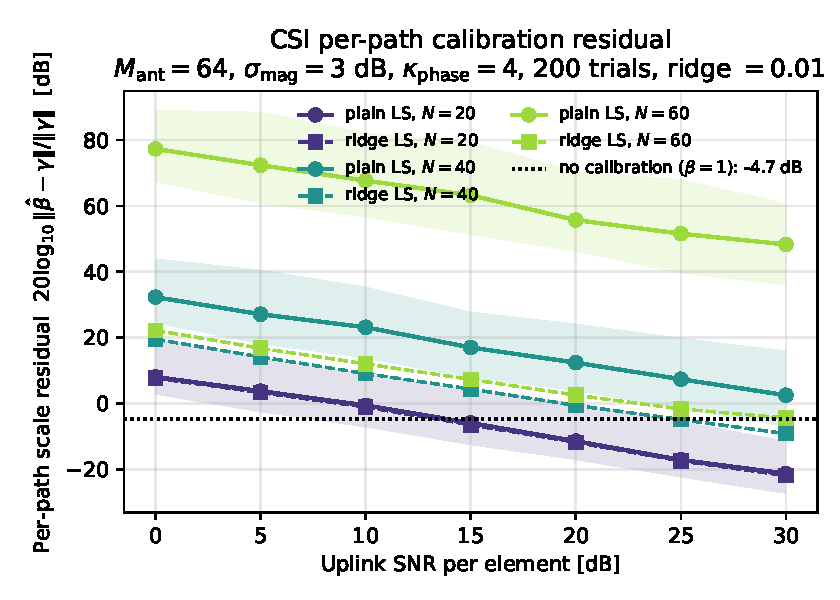
\includegraphics[width=\columnwidth]{residual_vs_snr.pdf}
  \caption{Per-path amplitude calibration residual versus uplink
  SNR, $M = 64$ array, three path counts. Plain LS (solid) versus
  ridge LS (dashed), median over 200 trials per cell. No-calibration
  baseline at $-4.7\,$dB. Ridge buys $25\,$dB at $N = 60$ near the
  array dimension, while plain LS converges only below $N \leq M/2$.}
  \label{fig:csi}
\end{figure}

\subsection{Cauchy bound on $\xx^H \Qmat^{(u)} \xx$
in the conditional regime}\label{sec:eval-cauchy}

A pose-agnostic upper bound on $\xx^H \Qmat^{(u)} \xx$ would let the
twin satisfy the budget without pose telemetry, by applying a
worst-case factor that depends only on the body's projected-area
geometry. The projected-area Cauchy formula gives the
direction-averaged absorbed power $\langle \Pabs \rangle =
\Sinc\,T_0\,\Aab/4$ for a convex body~\cite{Cauchy1841}, and a
peak-to-average directivity bound $D(\khat) \leq 2$ on the
projected-area-normalised intensity. The naive composition
$\xx^H \Qmat^{(u)} \xx \leq T_0\,(\Aab^{(u)}/4)\,D_{\max}^{(u)}\,
|\mathbf{a}_{\mathrm{BS}}^{(u)\,H} \xx|^2$, with
$\mathbf{a}_{\mathrm{BS}}$ the BS-side equivalent steering vector
to body $u$, holds only when $\xx$ is restricted to the steering
direction. \Cref{fig:tightness} measures the bound's tightness
over five precoder ensembles on Thelonious and Duke phantoms in both
path models. The mrt-LOS direction
($\xx \propto \mathbf{a}_{\mathrm{BS}}$) shows 21 to $27\,$dB of
slack and the bound holds by a wide margin. Random,
MRT-randomised, ECBF, and ZF-2-user precoders breach the bound
in 49 to $70\,\%$ of samples, with median ratios from $+2.86\,$dB
(iso-random, plaza-specular) to $+6.34\,$dB (ECBF, plaza-specular).
The mechanism is the inner product
$|\langle \mathbf{v}_1, \mathbf{a}_{\mathrm{BS}}/
\|\mathbf{a}_{\mathrm{BS}}\| \rangle|^2$ between the leading
exposure mode and the steering direction, which sits in
$[0.000, 0.19]$ across all evaluated jobs. The bound is useful
only when conditioned on a direction set that overlaps with
$\mathbf{a}_{\mathrm{BS}}$. \Cref{app:cauchy} states the conditional
form that does hold and proves it.

\begin{figure}[!t]
  \centering
  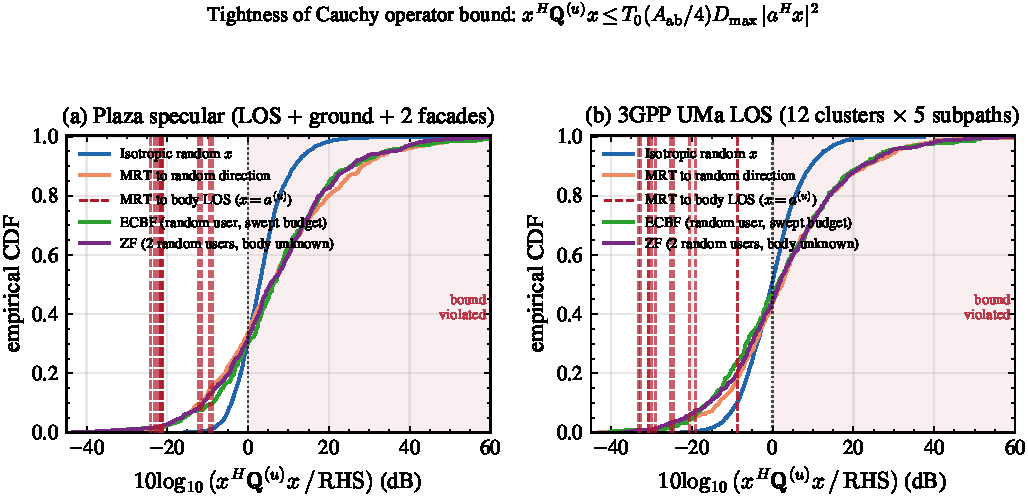
\includegraphics[width=\columnwidth]{tightness.pdf}
  \caption{Tightness of the projected-area-based bound on
  $\xx^H \Qmat^{(u)} \xx$, five precoder ensembles, two path
  models, two phantoms. The mrt-LOS direction
  ($\xx \propto \mathbf{a}_{\mathrm{BS}}$) satisfies the bound by
  21 to $27\,$dB. Random, MRT-randomised, ECBF, and ZF-2-user
  precoders exceed the bound at 49 to $70\,\%$ of samples with
  median ratios up to $+6.34\,$dB. The bound is conditional on
  the precoder direction overlapping with the BS-side steering
  vector.}
  \label{fig:tightness}
\end{figure}


\section{Regulatory framing}\label{sec:regulatory}

The closed loop has two regulatory pathways. The first is direct
audit of the basic restriction. ICNIRP 2020 specifies absorbed
power density above $6\,$GHz~\cite{ICNIRP2020}, and IEC/IEEE
$62232:2022$ prescribes an actual-exposure-scenario procedure for
fixed-site installations~\cite{IEC62232}. The per-body
$\Qmat^{(u)}$ construction is a first-principles evaluation of
absorbed power on a named anatomical mesh, conditioned on real
BS-side ray-traced channel state. A regulator can replay the
precoder-and-operator pair for any slot in the audit window and
recompute $\xx^H \Qmat^{(u)} \xx$ against the certificate. The
audit interface is open if the path dictionary, the body model, and
the dual variables are logged. The mechanism does not claim a
statutory exemption from the reference-level regime: it provides
direct compliance evidence under the basic-restriction pathway that
the standard already permits.

The second pathway is reference-level footprint reduction at
occupied public points. Brussels and Italy enforce reference levels
at all points reachable by the public~\cite{BrusselsArrete2007,ItalyDL}.
The proposed precoder reduces $\Pabs^{(u)}$ at every occupied $u$,
which strictly reduces the cumulative reference-level reading at
those points. The reading at unoccupied public points is governed by
the precoder's spatial coverage and is not affected by the
machinery. Combined with the chronic-dose ECDF of \cref{sec:chronic},
the deployment value is the chronic-dose reduction at occupied
points, not the slack instantaneous reading at unoccupied points.

The Brussels averaging window is $6\,$min in current
practice~\cite{BrusselsArrete2024}. The chronic-dose ECDF's
$5\,$min window covers most of one Brussels averaging window;
the integrated absorbed energy scales linearly with window length
under stationary load, so the tier-stratified ratios are
window-invariant. Italian attention values are $6\,$V/m on the
$24\,$h median outside dense urban centres under the 2024
decree~\cite{ItalyDL}; both regimes admit the same chronic-dose
argument with rescaled medians.


\section{Discussion}\label{sec:discussion}

The plaza evaluation answers a regime question. At $43\,$dBm
conducted transmit power and $E_{\mathrm{RL}} = 6\,$V/m, the
post-2014 Brussels arr\^et\'e and Italian outdoor attention level
for large urban areas, the per-body cap binds at every plaza-scale
deployment our path models support, and the precoder choice is
constrained on the cap. Geometric ZF gives the highest
unconstrained sum-rate ($44\,$Gbps mean over the 5-min trace) at
$16.7\,\%$ violation rate; MRT gives $11\,$Gbps at $35.1\,\%$
violation; the proposed multi-body WMMSE-ECBF closes the cap at
$1.0\%$ violation under oracle pose and $2.5\%$ under deployed
virtual-IMU pose, paying for compliance with sum-rate. The
closed-loop machinery becomes load-bearing inside this corner, and
the rest of the regulatory landscape — the current Brussels
$14.57\,$V/m cumulative cap, the Italian $15\,$V/m exposure
category for low-density areas, and the $30\,$dBm conducted-power
band — sits in slack regimes where any reasonable precoder satisfies
the cap by orders of magnitude. The chronic-dose ECDF separates the
tiers and is the regulator-facing readback of the loop, surviving
both regimes.

The pose-information triage of \cref{sec:eval-imu} is the most
operationally interesting result. Pose telemetry shapes
$\Qmat^{(u)}(\bm\theta)$ by aligning the leading eigenvector with
the body's torso plane. The closed-form precoder converts that
shaping into a tighter feasible cone in the $\bm\lambda$ direction.
Tighter feasible cone means more frequent solver fallback under the
$\textsf{max\_outer} = 8$ Newton cap, but lower realised exposure
on the slots where the solver converges. The trade-off is
solver-side, not physical: the IMU pose at $4^\circ$
$\sigma_{\mathrm{joint}}$ buys $1.8\times$ compliance over Cauchy
envelope at $76\%$ fallback versus $55\%$ fallback. Uncapping the
inner sweep, switching to a low-rank $\Qmat^{(u)}$ Cholesky path
that already lands in the implementation, and replacing the
Cauchy-on-tier-C envelope with a Lanczos-projected operator are
the three direct follow-ups; each shrinks the fallback rate at
proportional per-slot wall-clock cost. The slot wall-clock budget
is set by the PHY frame rate and the body-population GPU
throughput; at the binding regime ($M = 64$, $K = B = 25$, JAX
backend on RTX 4090), the median solve is $116\,$ms and the
$95^{\mathrm{th}}$ percentile is $\sim 800\,$ms. The
operationally-correct path is to schedule the inner sweep
across slots and accept a per-slot delay, which the body-motion
cadence ($\sim 1\,$s for $1\,$m of displacement) tolerates.

The bound discussion is sharper than expected. The naive
projected-area bound on $\xx^H \Qmat^{(u)} \xx$ that the literature
sometimes invokes is not a universal upper bound. It holds for $\xx$
in the BS-side steering direction by a 21 to $27\,$dB margin and
fails at 49 to $70\,\%$ of random and ECBF precoders. The
conditional form in \cref{app:cauchy} is the right object to use:
the bound applies over a chosen direction set, and the worst case
over that set is what the twin commits to. The mechanism, that the
leading exposure mode does not align with the BS-side steering
vector, is a geometric fact about how a body couples to a
$64$-element panel and is worth flagging in any compliance-bound
construction that does not condition on the direction.

The empirical Q-rank result has a related geometric content. With
the panel resolving $\sim 14^\circ$ in azimuth at $26\,$GHz and the
body subtending several beams across its torso, the dominant body
modes condense into 3 to 4 distinguishable beam directions
regardless of multipath density. This is a panel-side affordance,
not a model simplification, and it makes the closed-form solver
inexpensive on $\Qmat_{\mathrm{tot}}$. Adding multipath through
denser ray-tracing or higher-order reflections raises the trace but
not the rank.

The present evaluation has four limitations. First, the PHY surrogate
is Shannon capacity rather than Sionna NR PHY. A calibrated
modulation-coding-scheme link curve would shift the absolute
sum-rate numbers but should not affect the violation/sum-rate
trade-off. Second, the $5\,$min steady-state window is a single seed;
multi-seed averaging would smooth the chronic-dose ECDF tails further.
Third, the ZF baseline is naive (singular $\hh \hh^H$ at $K = 25$ in
UMa-LOS). A regularised ZF would not collapse, and the comparison is
informative only as a degeneracy boundary. Fourth, the IMU model is
a calibrated Madgwick/xsens proxy; a deep-learning-augmented
inertial-mocap pipeline would lower $\sigma_{\mathrm{joint}}$ to the
$1.5^\circ$ floor of \cref{fig:imu-sweep}. None of these affect the
qualitative conclusions.

The closed-loop architecture extends in three directions naturally.
A cooperative multi-operator allocation generalises the per-body
budget $L^{(u)}$ to a cumulative cap shared across operators in the
same band, with each operator's twin seeing its own slot of the
cumulative budget. A pose-differentiable
$\Qmat^{(u)}(\bm\theta)$ closes the loop on tier-A bodies under
near-field user-equipment exposure where the leading mode's azimuth
depends strongly on torso orientation. A reflective intelligent
surface in the binding-regime corner can buy back the cap by
redirecting power along geometrically chosen paths, which is a
one-line modification to the $\Mmat^{(u)}$ Gram in
\cref{eq:Q-factor}.


\section{Conclusion}\label{sec:conclusion}

A body-side digital twin in the multi-user mmWave precoder loop is
constructible from three ingredients that the network already
maintains. A coherent exposure operator
$\Qmat^{(u)} = \Jmat^T\,\Mmat^{(u)}\,\Jmat$ comes from the same
ray-traced path set that gives the user-equipment channel. A scene
path dictionary precomputed offline, indexed by body position, and
calibrated at runtime by ridge least squares against served-user
uplink CSI, supplies $\Mmat^{(u)}$ without per-slot ray tracing. A
multi-user QCQP under per-body exposure caps admits the WMMSE-driven
closed form
$\ww_k^\star = (\Qmat_{\mathrm{tot}} + \Hintf + \nu \mathbf{I})^{-1}
u_k v_k\,\hh_k^*$, generalising regularised zero-forcing on the
heterogeneous user-and-bystander steering set. A virtual-IMU pose
estimator with calibrated bias drift and accelerometer corrector
gives the loop tier-A and tier-B SMPL pose at the
$\sim 100\,$ms cadence pose actually changes; tier-C bystanders
default to the projected-area Cauchy envelope. The loop runs at the
cadences the network already sustains: $1\,$ms PHY, $\sim 100\,$ms
pose update, $\sim 1\,$s translation phasor, offline ray tracing
and dictionary calibration.

We instantiate the loop at plaza scale on 50 SMPL-X bodies under
$26\,$GHz $8 \times 8$ panel illumination at the post-2014 Brussels
arr\^et\'e and Italian outdoor attention level
$E_{\mathrm{RL}} = 6\,$V/m, $43\,$dBm conducted. The empirical
operator rank is 3 to 4 at the $99\,\%$ trace fraction; geometric
ZF and MRT violate the cap on $16.7\,\%$ and $35.1\,\%$ of
body-slots respectively over the 5-min steady-state walk; the
proposed multi-body WMMSE-ECBF holds the cap on $99.0\,\%$ of
body-slots under ground-truth pose, on $97.5\,\%$ under virtual-IMU
pose at $4^\circ$ steady-state per-joint attitude RMS, and on
$95.4\,\%$ under T-pose Cauchy envelope; the chronic-dose
ECDF separates served, cooperating, and bystander tiers by
$1.5\times$. The standard projected-area bound on
$\xx^H \Qmat^{(u)} \xx$ is loose by 21 to $27\,$dB on the steering
direction and breached by 49 to $70\,\%$ of unconstrained
precoders, which we trace to the geometric mismatch between the
leading exposure mode and the BS-side steering vector. The
conditional bound that does hold is the one to use in
compliance-aware precoder design.


\appendices

\section{Per-path Fresnel transmission operator}\label{app:fresnel}

The per-path Fresnel transmission operator $\Fn(\rr)$ in
\cref{eq:psitil} maps the incident polarisation amplitude $\psin$
to its TE-and-TM-filtered counterpart on the body surface. At a
surface point $\rr$ with outward normal $\nhat$, path $n$ has
incidence cosine $\mu_n = \nhat \cdot (-\khat_n)$. For $\mu_n > 0$,
the local TE and TM unit vectors are
$\hat{e}_{s,n} = \khat_n \times \nhat / |\khat_n \times \nhat|$ and
$\hat{e}_{p,n} = \hat{e}_{s,n} \times \khat_n$. The Fresnel
amplitude transmission coefficients are
\begin{equation}\label{eq:t-coef-app}
  t_{s,n} = \frac{2 \mu_n}{\mu_n + \xi_n},
  \qquad
  t_{p,n} = \frac{2 \ntilde \mu_n}{\ntilde^2 \mu_n + \xi_n},
\end{equation}
with $\xi_n = \sqrt{\ntilde^2 - 1 + \mu_n^2}$ and
$\RE(\xi_n) > 0$. The operator acts as
\begin{equation}\label{eq:F-action}
  \Fn(\rr)\,\psin = t_{s,n}(\hat{e}_{s,n} \cdot \psin)
  \hat{e}_{s,n} + t_{p,n}(\hat{e}_{p,n} \cdot \psin) \hat{e}_{p,n},
\end{equation}
on a front-facing path. Back-facing paths ($\mu_n < 0$) contribute
zero. The depth-decay coefficient is
$\alpha_n^{(d)} = -k_0\,\IM(\xi_n)$. The two cross-term
approximations of \cref{sec:cohlaw} hold uniformly in incidence
angle and bound the cross-term error on $\Sab$ at $\leq 5\,\%$ for
any precoder.


\section{WMMSE-ECBF dual problem}\label{app:ecbf}

The closed-form precoder of \cref{eq:closedform} arises from the
WMMSE surrogate of the multi-user sum-rate problem. With
$y_k(\xx) = \hh_k^T \xx$, the per-stream MSE
\begin{equation}
  e_k = |1 - v_k^* \hh_k^T \ww_k|^2 + |v_k|^2 \sigma_n^2 +
  |v_k|^2 \sum_{k' \neq k} |\hh_k^T \ww_{k'}|^2
\end{equation}
and the WMMSE objective
$\tilde R(\{\ww_k\}) = \sum_k\bigl[\log u_k - u_k\,e_k +
\mathrm{const.}\bigr]$. The Lagrangian for $\ww_k$ under the
exposure and power constraints is
\begin{equation}\label{eq:lagrangian}
\begin{aligned}
\mathcal{L}({\ww_k}, \bm\lambda, \nu)
={}& -\tilde R + \sum_u \lambda_u
  \biggl(\sum_k \ww_k^H \Qmat^{(u)} \ww_k - L^{(u)}\biggr) \\
& + \nu\biggl(\sum_k \|\ww_k\|^2 - P_{\mathrm{tx}}\biggr).
\end{aligned}
\end{equation}
Stationarity in $\ww_k$, fixing $u_k, v_k$ at the inner WMMSE
optima of \cref{eq:uv-update}, gives
\begin{equation}\label{eq:KKT}
  \bigl(\Qmat_{\mathrm{tot}}(\bm\lambda) + \Hintf + \nu\,
  \mathbf{I}\bigr) \ww_k = u_k v_k \hh_k^*,
\end{equation}
which is \cref{eq:closedform}. The dual variables
$(\bm\lambda, \nu)$ are updated by Newton ascent on the dual
residual
$F_u(\bm\lambda, \nu) = \sum_k \ww_k^{\star\,H}(\bm\lambda, \nu)
\Qmat^{(u)} \ww_k^\star - L^{(u)}$ for $\bm\lambda$ and bisection
on $\nu$ for the power constraint. The dual-feasibility set is the
positive orthant intersected with the budget hyperplanes. In our
implementation, the WMMSE outer iteration terminates in 4 to 8
sweeps from a cold start, with warm-starting across slots reducing
this to $\sim 3$ sweeps. The inner inverse in
\cref{eq:closedform} is $M \times M$ Cholesky-solvable at $O(M^3)$
once per outer iteration. For $K = B = 25$ and $M = 64$ at the
binding regime, the median wall-clock is $116\,$ms per slot on a
single-thread JAX backend on RTX 4090 with the body-batch
finite-difference Jacobian fanned out under \texttt{jax.vmap},
under the production cap $\textsf{max\_outer} = 8$.


\section{Conditional Cauchy bound}\label{app:cauchy}

The projected-area bound on $\xx^H \Qmat^{(u)} \xx$ holds only
when the precoder is restricted to a chosen BS-side direction set.

\begin{theorem}[Conditional projected-area bound]\label{thm:cauchy-cond}
Let $\Qmat^{(u)}$ be the per-body exposure operator at body $u$
and let $\mathcal{A} \subseteq \Complex^M$ be a closed direction
set containing the BS-side equivalent steering vector
$\mathbf{a}_{\mathrm{BS}}^{(u)}$. For any precoder $\xx$ that lies
in the conic hull of $\mathcal{A}$,
\begin{equation}\label{eq:cauchy-cond}
  \xx^H \Qmat^{(u)} \xx \leq T_0\,\frac{\Aab^{(u)}}{4}\,
  D_{\max}^{(u)}\;\sup_{\mathbf{a} \in \mathcal{A}}
  |\mathbf{a}^H \xx|^2,
\end{equation}
where $\Aab^{(u)} = \int_{\Sigma^{(u)}} \eta(\rr)\,\diff A$ is the
absorption area, $\eta \in [0,1]$ is the ambient-occlusion factor,
$T_0 = 4 n / ((n+1)^2 + \kappa^2)$ is the normal-incidence Fresnel
transmittance, and $D_{\max}^{(u)} = \max_{\khat}
4\,A_\perp^{(u)}(\khat)/\Aab^{(u)}$ is the body's peak
projected-area-normalised directivity. For convex bodies
$D_{\max}^{(u)} \leq 2$.
\end{theorem}

\begin{proof}
By the angular-spectrum decomposition,
$\xx^H \Qmat^{(u)} \xx = \int_{S^2} D(\khat;\bm\theta_u)\,
|\bm\alpha_{\mathrm{BS}}^{(u)}(\khat)^H \xx|^2\,\diff\Omega$,
with $D(\khat;\bm\theta_u) = 4 A_\perp^{(u)}(\khat)/\Aab^{(u)}$
the direction-resolved directivity at pose $\bm\theta_u$ and
$\bm\alpha_{\mathrm{BS}}^{(u)}(\khat)$ the BS-side path-amplitude
vector for arrival direction $\khat$ on body $u$. Restricting to
$\xx$ in the conic hull of $\mathcal{A}$ bounds the inner product
by $\sup_{\mathbf{a} \in \mathcal{A}} |\mathbf{a}^H \xx|^2$.
Bounding $D \leq D_{\max}^{(u)}$ uniformly and integrating over
the sphere $\int_{S^2} \diff\Omega = 4\pi$ together with the
Cauchy projected-area identity
$\int_{S^2} A_\perp^{(u)}(\khat)\,\diff\Omega/4\pi =
\Aab^{(u)}/4$ gives the stated bound, with the factor $T_0$
accounting for the normal-incidence Fresnel transmittance.
\end{proof}

\Cref{thm:cauchy-cond} is the bound the twin uses when it does not
have pose telemetry. The direction set $\mathcal{A}$ is chosen as
the BS-side beamforming codebook restricted to the body's spatial
sector. The bound is loose in proportion to the geometric mismatch
between $\mathbf{a}_{\mathrm{BS}}^{(u)}$ and the leading exposure
eigenvector $\mathbf{v}_1$, which the empirical measurement of
\cref{sec:eval-cauchy} places at
$|\langle \mathbf{v}_1, \mathbf{a}_{\mathrm{BS}}/
\|\mathbf{a}_{\mathrm{BS}}\| \rangle|^2 \in [0.000, 0.19]$ on the
Thelonious and Duke phantoms. A precoder constructed outside the
conic hull of $\mathcal{A}$ is not bounded by \cref{eq:cauchy-cond};
the twin must fall back to the full $\xx^H \Qmat^{(u)} \xx$
evaluation.


\bibliographystyle{IEEEtran}
\bibliography{../../papers/drafts/refs}

\end{document}
